\documentclass[aspectratio=169,professionalfonts]{beamer}

\usepackage[T1]{fontenc}
\usepackage[utf8]{inputenc}
\usepackage{lmodern}
\usepackage{amsmath,amssymb,bm,mathtools}
\usepackage{booktabs}
\usepackage{tikz}
\usepackage{array}
\usepackage{multicol}
\usepackage{hyperref}
\usepackage{xcolor}
\usepackage{appendixnumberbeamer}

% ---------- Colors ----------
\definecolor{navy}{HTML}{123B63}
\definecolor{teal}{HTML}{1F8A8A}
\definecolor{sky}{HTML}{EAF4FB}
\definecolor{mint}{HTML}{E8F6F4}
\definecolor{textgray}{HTML}{263238}
\definecolor{lightline}{HTML}{D7E3EC}
\definecolor{softgray}{HTML}{F6F8FB}
\definecolor{accent2}{HTML}{4AA3D9}
\definecolor{warn}{HTML}{A94E00}

\setbeamercolor{normal text}{fg=textgray,bg=white}
\setbeamercolor{frametitle}{fg=navy,bg=white}
\setbeamercolor{title}{fg=navy}
\setbeamercolor{subtitle}{fg=teal}
\setbeamercolor{structure}{fg=teal}
\setbeamercolor{block title}{fg=white,bg=navy}
\setbeamercolor{block body}{fg=textgray,bg=sky}
\setbeamercolor{block title alerted}{fg=white,bg=teal}
\setbeamercolor{block body alerted}{fg=textgray,bg=mint}
\setbeamercolor{itemize item}{fg=teal}
\setbeamercolor{itemize subitem}{fg=accent2}

\setbeamertemplate{navigation symbols}{}
\setbeamertemplate{blocks}[rounded][shadow=false]
\setbeamertemplate{itemize items}[circle]
\setbeamertemplate{enumerate items}[default]

% ---------- Footer / header ----------
\newcommand{\deckbrand}{CTMC}
\setbeamerfont{footline}{size=\scriptsize}
\setbeamerfont{frametitle}{series=\bfseries,size=\Large}
\setbeamerfont{title}{series=\bfseries,size=\LARGE}
\setbeamerfont{subtitle}{size=\large}

\setbeamertemplate{headline}{%
  \begin{beamercolorbox}[wd=\paperwidth,ht=0.18cm,dp=0cm]{normal text}
    \color{teal}\rule{\paperwidth}{0.18cm}
  \end{beamercolorbox}%
}

\setbeamertemplate{footline}{%
  \leavevmode%
  \hbox{%
    \begin{beamercolorbox}[wd=.78\paperwidth,ht=0.34cm,dp=0.12cm,leftskip=0.35cm]{author in head/foot}%
      {\color{navy}\deckbrand}
    \end{beamercolorbox}%
    \begin{beamercolorbox}[wd=.22\paperwidth,ht=0.34cm,dp=0.12cm,rightskip=0.35cm plus1fil]{date in head/foot}%
      {\color{navy}\insertframenumber/\inserttotalframenumber}
    \end{beamercolorbox}%
  }%
  \begin{beamercolorbox}[wd=\paperwidth,ht=0.10cm,dp=0cm]{normal text}
    \color{accent2}\rule{\paperwidth}{0.10cm}
  \end{beamercolorbox}%
}

% ---------- Helpers ----------
\newcommand{\Prob}{\mathbb{P}}
\newcommand{\E}{\mathbb{E}}
\newcommand{\dd}{\,\mathrm{d}}
\newcommand{\ind}{\mathbf{1}}
\newcommand{\R}{\mathbb{R}}

\newcolumntype{L}[1]{>{\raggedright\arraybackslash}p{#1}}
\newcolumntype{C}[1]{>{\centering\arraybackslash}p{#1}}

\title{Lecture 7 Pre-CTMC}
\subtitle{From short-time transition rules to exponential holding times}
\author{Course notes}
\date{}

\begin{document}

\begin{frame}[plain]
  \vspace{0.25cm}
  {\color{navy}\bfseries\LARGE Lecture 7 Pre-CTMC\par}
  \vspace{0.12cm}
  {\color{teal}\large From short-time transition rules to exponential holding times\par}
  \vspace{0.28cm}
  \centering
  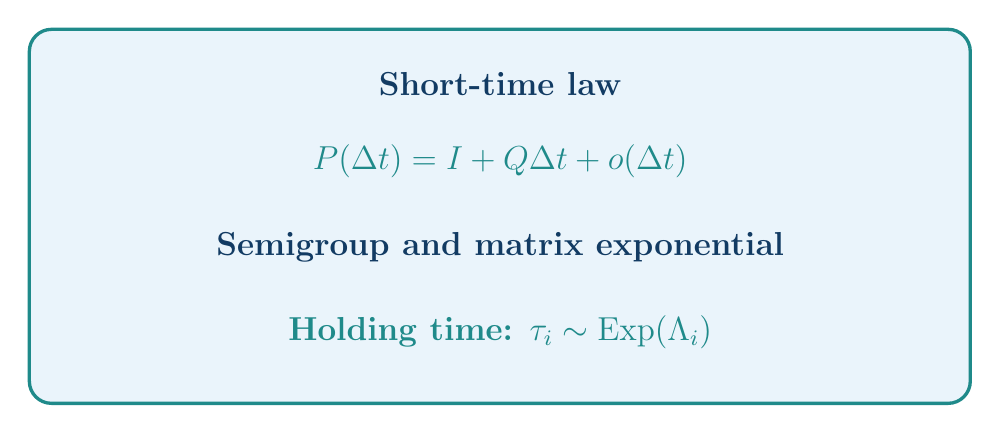
\begin{tikzpicture}[x=1cm,y=1cm]
    \fill[sky,rounded corners=8pt] (0,0) rectangle (11.95,4.75);
    \draw[teal,line width=1.2pt,rounded corners=8pt] (0,0) rectangle (11.95,4.75);
    \node[text=navy,font=\large\bfseries] at (5.98,4.05) {Short-time law};
    \node[text=teal,font=\large\bfseries] at (5.98,3.08) {$P(\Delta t)=I+Q\Delta t+o(\Delta t)$};
    \node[text=navy,font=\large\bfseries] at (5.98,1.98) {Semigroup and matrix exponential};
    \node[text=teal,font=\large\bfseries] at (5.98,0.90) {Holding time: $\tau_i \sim \mathrm{Exp}(\Lambda_i)$};
  \end{tikzpicture}
  \vspace{0.12cm}

  {\color{navy}\small A reorganized version following the board derivation: local transition probabilities, generator, semigroup, and first jump time.}
\end{frame}

\begin{frame}{Roadmap}
\small
\begin{block}{Goal}
Starting from the local short-time transition probabilities of a continuous-time Markov chain, we will first identify the generator entries from limits, then derive the matrix evolution law, and finally study the first jump time from a fixed state.
\end{block}

\begin{columns}[T,totalwidth=\textwidth]
\column{0.49\textwidth}
\begin{alertblock}{Part I: Global transition law}
\begin{enumerate}
  \item short-time probabilities with rates $\lambda_{ij}$
  \item define $q_{ij}$ and $q_{ii}$ from limits
  \item only then write the matrix forms for $P(t)$ and $Q$
\end{enumerate}
\end{alertblock}

\column{0.49\textwidth}
\begin{block}{Part II: When to jump}
\begin{enumerate}
  \item define the first jump time $\tau_i$
  \item derive its survival function
  \item obtain density and mean waiting time
\end{enumerate}
\end{block}
\end{columns}
\end{frame}

\begin{frame}{Short-time transition assumption}
\small
Let the state space be a countable set $I=\{0,1,2,\dots\}$.
For a CTMC, the future depends only on the current state.

\vspace{0.15cm}
\begin{block}{Local transition rule at state $i$}
For $j\neq i$, in a very short interval $\Delta t$,
\[
\Prob(X_{t+\Delta t}=j\mid X_t=i)=\lambda_{ij}\Delta t+o(\Delta t).
\]
Hence the probability of staying at $i$ is
\[
\Prob(X_{t+\Delta t}=i\mid X_t=i)
=1-\sum_{j\neq i}\lambda_{ij}\Delta t+o(\Delta t).
\]
\end{block}

\begin{alertblock}{Notation}
Define the total leaving rate
\[
\Lambda_i:=\sum_{j\neq i}\lambda_{ij}.
\]
Then
\[
\Prob(X_{t+\Delta t}=i\mid X_t=i)=1-\Lambda_i\Delta t+o(\Delta t).
\]
\end{alertblock}
\end{frame}

\begin{frame}{From $\lambda_{ij}$ to $q_{ij}$}
\scriptsize
\begin{block}{Off-diagonal terms}
For $j\neq i$,
\[
\frac{\Prob(X_{t+\Delta t}=j\mid X_t=i)-\Prob(X_t=j\mid X_t=i)}{\Delta t}
=\frac{\lambda_{ij}\Delta t+o(\Delta t)-0}{\Delta t}.
\]
Taking $\Delta t\to 0$ gives
\[
q_{ij}=\lambda_{ij},\qquad j\neq i.
\]
\end{block}

\begin{alertblock}{Diagonal term}
\[
q_{ii}
=\lim_{\Delta t\to 0}
\frac{\Prob(X_{t+\Delta t}=i\mid X_t=i)-1}{\Delta t}.
\]
Using
\[
\Prob(X_{t+\Delta t}=i\mid X_t=i)=1-\Lambda_i\Delta t+o(\Delta t),
\]
we obtain
\[
q_{ii}=-\Lambda_i=-\sum_{j\neq i}\lambda_{ij}.
\]
\end{alertblock}
\end{frame}

\begin{frame}{Only now introduce the generator matrix}
\scriptsize
After defining the entries one by one, collect them into the generator
\[
Q=(q_{ij}).
\]
The entrywise short-time formulas become
\[
\Prob(X_{t+\Delta t}=j\mid X_t=i)=q_{ij}\Delta t+o(\Delta t),\qquad j\neq i,
\]
and
\[
\Prob(X_{t+\Delta t}=i\mid X_t=i)=1+q_{ii}\Delta t+o(\Delta t).
\]

\begin{block}{Generator structure}
\[
q_{ij}\ge 0\ (j\neq i),\qquad
q_{ii}=-\sum_{j\neq i}q_{ij}.
\]
\end{block}

\begin{alertblock}{Why this is intuitive}
Off-diagonal entries are jump rates to other states. The diagonal entry is exactly what is needed so that each row still sums to $1$ to first order.
\end{alertblock}
\end{frame}

\begin{frame}{The infinitesimal form of the transition matrix}
\small
Now define the finite-time transition probabilities
\[
P_{ij}(t):=\Prob(X_t=j\mid X_0=i).
\]
Combining the diagonal and off-diagonal cases gives
\[
P_{ij}(\Delta t)=\delta_{ij}+q_{ij}\Delta t+o(\Delta t).
\]
In matrix form,
\[
P(\Delta t)=I+Q\Delta t+o(\Delta t),
\]
where $Q=(q_{ij})$ is the generator matrix.

\begin{block}{Interpretation}
The matrix form is just a compact summary of the entrywise limits:
\begin{itemize}
  \item off-diagonal entries record where the chain can jump,
  \item diagonal entries record how quickly the chain leaves the current state.
\end{itemize}
\end{block}
\end{frame}

\begin{frame}{Matrix differential equation}
\small
By the Markov property,
\[
P(t+\Delta t)=P(t)\,P(t+\Delta t\mid t).
\]
Time-homogeneity implies
\[
P(t+\Delta t\mid t)=P(\Delta t).
\]
Hence
\[
P(t+\Delta t)=P(t)P(\Delta t)=P(t)\bigl(I+Q\Delta t+o(\Delta t)\bigr).
\]

Rearranging,
\[
\frac{P(t+\Delta t)-P(t)}{\Delta t}=P(t)Q+o(1).
\]
Letting $\Delta t\to 0$,
\[
P'(t)=P(t)Q.
\]

\begin{alertblock}{Kolmogorov equation in matrix form}
With initial condition $P(0)=I$,
\[
P'(t)=P(t)Q,\qquad P(0)=I.
\]
\end{alertblock}

\begin{block}{Terminology note}
In many textbooks, $P'(t)=P(t)Q$ is called the \emph{backward} equation, while
\[
P'(t)=QP(t)
\]
is called the \emph{forward} equation. For a time-homogeneous finite-state CTMC, both matrix equations hold under the usual setting.
\end{block}
\end{frame}

\begin{frame}{Why the solution is $P(t)=e^{tQ}$}
\small
Consider the matrix exponential
\[
e^{tQ}:=\sum_{n=0}^{\infty}\frac{(tQ)^n}{n!}.
\]
Differentiate term by term:
\[
\frac{\dd}{\dd t}e^{tQ}
=Q\sum_{n=0}^{\infty}\frac{t^nQ^n}{n!}
=e^{tQ}Q.
\]
Also,
\[
e^{0Q}=I.
\]
Therefore $e^{tQ}$ solves the same differential equation and initial condition:
\[
P'(t)=P(t)Q,\qquad P(0)=I.
\]

\begin{block}{Conclusion}
\[
P(t)=e^{tQ}.
\]
This is the global transition law obtained from the local generator $Q$.
\end{block}
\end{frame}

\begin{frame}{An equivalent discrete-time approximation}
\small
From
\[
P(\Delta t)=I+Q\Delta t+o(\Delta t),
\]
one can iterate over many tiny steps:
\[
P(t)\approx \bigl(I+Q\tfrac{t}{n}\bigr)^n.
\]
Letting $n\to\infty$ gives
\[
P(t)=\lim_{n\to\infty}\bigl(I+Q\tfrac{t}{n}\bigr)^n=e^{tQ}.
\]

\begin{alertblock}{Meaning}
This matches the intuition from the board derivation:
many infinitesimal updates combine into the matrix exponential.
\end{alertblock}
\end{frame}

\begin{frame}{Two important consequences of $P(t)=e^{tQ}$}
\small
\begin{block}{1. Do not read $e^{tQ}$ entrywise}
In general,
\[
P_{ii}(t)\neq e^{t q_{ii}}.
\]
The expression $e^{tQ}$ is a \textbf{matrix exponential}, not an entrywise exponential.
\end{block}

\begin{alertblock}{2. Probability is conserved}
Because each row of $Q$ sums to zero,
\[
Q\mathbf 1=0.
\]
Hence
\[
P(t)\mathbf 1=e^{tQ}\mathbf 1=\mathbf 1.
\]
So every row of $P(t)$ sums to $1$, exactly as a transition matrix should.
\end{alertblock}
\end{frame}

\begin{frame}{Now ask a different question: when to jump?}
\small
Fix a state $i$ and assume the chain starts there:
\[
X_0=i.
\]
Define the first jump time from state $i$ by
\[
\tau_i:=\inf\{t>0:X_t\neq i\}.
\]

\begin{block}{Important distinction}
\[
\Prob(\tau_i>t\mid X_0=i)
\]
means the chain has stayed at $i$ during the entire interval $[0,t]$.

This is stronger than merely saying $X_t=i$, because the chain could leave and return.
\end{block}
\end{frame}

\begin{frame}{Survival function of the first jump time}
\small
Let
\[
S_i(t):=\Prob(\tau_i>t\mid X_0=i).
\]
To survive up to time $t+\Delta t$, the chain must:
\begin{enumerate}
  \item survive up to time $t$;
  \item then stay at $i$ during $[t,t+\Delta t]$.
\end{enumerate}

Hence
\[
S_i(t+\Delta t)=S_i(t)\bigl(1-\Lambda_i\Delta t+o(\Delta t)\bigr).
\]
Therefore
\[
\frac{S_i(t+\Delta t)-S_i(t)}{\Delta t}
=-\Lambda_i S_i(t)+o(1).
\]
Letting $\Delta t\to 0$ yields
\[
S_i'(t)=-\Lambda_i S_i(t),\qquad S_i(0)=1.
\]
So
\[
S_i(t)=e^{-\Lambda_i t}.
\]
\end{frame}

\begin{frame}{The law of the waiting time}
\small
From the survival function,
\[
\Prob(\tau_i>t\mid X_0=i)=e^{-\Lambda_i t}.
\]
Hence the cumulative distribution function is
\[
\Prob(\tau_i\le t\mid X_0=i)=1-e^{-\Lambda_i t}.
\]
Differentiating,
\[
f_{\tau_i}(t)=\Lambda_i e^{-\Lambda_i t},\qquad t\ge 0.
\]

\begin{columns}[T,totalwidth=\textwidth]
\column{0.48\textwidth}
\begin{block}{Density}
\[
f_{\tau_i}(t)=\Lambda_i e^{-\Lambda_i t}.
\]
This is exactly the density of an exponential law with parameter $\Lambda_i$.
\end{block}

\column{0.48\textwidth}
\begin{alertblock}{Equivalent small-window form}
\[
\Prob(t\le \tau_i\le t+\Delta t)
\approx e^{-\Lambda_i t}\Lambda_i\Delta t.
\]
Survival up to $t$ times jump in the next tiny interval.
\end{alertblock}
\end{columns}
\end{frame}

\begin{frame}{CDF, density, and the correct small-window reading}
\scriptsize
The key small-window interpretation is
\[
\Prob(t\le \tau_i<t+\Delta t)\approx f_{\tau_i}(t)\,\Delta t.
\]
So once we know the density, we know the probability of the first jump landing near time $t$.

\vspace{0.05cm}
Since
\[
\Prob(\tau_i>t)=e^{-\Lambda_i t},
\]
the CDF is
\[
F_{\tau_i}(t)=\Prob(\tau_i\le t)=1-e^{-\Lambda_i t},
\qquad t\ge 0,
\]
and the density is
\[
f_{\tau_i}(t)=\Lambda_i e^{-\Lambda_i t}.
\]

\begin{columns}[T,totalwidth=\textwidth]
\column{0.50\textwidth}
\begin{block}{Important clarification}
For a continuous random variable,
\[
\Prob(\tau_i=t)=0.
\]
So $f_{\tau_i}(t)$ is not the probability of jumping \emph{exactly} at time $t$.
\end{block}

\column{0.46\textwidth}
\begin{alertblock}{Correct interpretation}
For small $\Delta t$,
\[
\Prob(t\le \tau_i<t+\Delta t)
\approx f_{\tau_i}(t)\,\Delta t.
\]
It describes the probability of the first jump landing in a tiny interval around $t$.
\end{alertblock}
\end{columns}
\end{frame}

\begin{frame}{A useful factorization of the density}
\small
The formula
\[
\Prob(t\le \tau_i<t+\Delta t)\approx e^{-\Lambda_i t}\Lambda_i\Delta t
\]
has a very clean interpretation:
\[
\underbrace{e^{-\Lambda_i t}}_{\substack{\text{survive until }t\\\text{(no jump yet)}}}
\times
\underbrace{\Lambda_i\Delta t}_{\substack{\text{jump during the next}\\\text{tiny interval}}}.
\]
Therefore
\[
f_{\tau_i}(t)=S_i(t)\cdot \Lambda_i.
\]

\begin{block}{What changes between the two probabilities?}
\begin{itemize}
  \item $\Lambda_i\Delta t$: probability of a jump in the next tiny interval, given that we are still in state $i$ now.
  \item $\Lambda_i e^{-\Lambda_i t}\Delta t$: probability that the \emph{first} jump occurs near time $t$.
\end{itemize}
\end{block}
\end{frame}

\begin{frame}{Mean waiting time}
\small
Since
\[
\tau_i\sim \mathrm{Exp}(\Lambda_i),
\]
its expectation is
\[
\E[\tau_i]
=\int_0^\infty t\,\Lambda_i e^{-\Lambda_i t}\,\dd t
=\frac{1}{\Lambda_i}.
\]

\begin{block}{Interpretation}
The total leaving rate $\Lambda_i$ determines how long the chain typically stays in state $i$:
\[
\text{large }\Lambda_i \Longrightarrow \text{short waiting time},\qquad
\text{small }\Lambda_i \Longrightarrow \text{long waiting time}.
\]
\end{block}
\end{frame}

\begin{frame}{Equivalent interpretations of the exponential law}
\scriptsize
\begin{columns}[T,totalwidth=\textwidth]
\column{0.48\textwidth}
\begin{block}{Time scale}
\[
\E[\tau_i]=\frac{1}{\Lambda_i},
\qquad
\mathrm{Var}(\tau_i)=\frac{1}{\Lambda_i^2}.
\]
The parameter $\Lambda_i$ sets the natural residence-time scale of state $i$.
\end{block}

\begin{alertblock}{Memoryless property}
\[
\Prob(\tau_i>s+t\mid \tau_i>s)=\Prob(\tau_i>t).
\]
After already waiting for time $s$, the remaining waiting time has the same law as before.
\end{alertblock}

\column{0.48\textwidth}
\begin{block}{Hazard interpretation}
\[
\lambda_{\mathrm{haz}}(t)=\frac{f_{\tau_i}(t)}{S_i(t)}=\Lambda_i.
\]
The instantaneous leaving intensity is constant as long as the chain is still at $i$.
\end{block}

\begin{alertblock}{Conceptual meaning}
The state $i$ does not remember how long it has already been occupied; only the current state matters.
\end{alertblock}
\end{columns}
\end{frame}

\begin{frame}{``When to jump'' and ``where to jump'' are different objects}
\small
The outgoing rates from state $i$ contain two different pieces of information.

\begin{block}{1. When to jump}
\[
\tau_i\sim \mathrm{Exp}(\Lambda_i),
\qquad
\Lambda_i=\sum_{j\neq i}q_{ij}.
\]
Only the \textbf{sum} of outgoing rates matters for the holding time.
\end{block}

\begin{alertblock}{2. Where to jump}
Conditioned on the event that a jump occurs, the destination is
\[
\Prob(X_{\tau_i}=j\mid X_0=i,\text{ jump occurs})
=\frac{q_{ij}}{\Lambda_i},\qquad j\neq i.
\]
Only the \textbf{relative proportions} of the off-diagonal rates matter.
\end{alertblock}
\end{frame}

\begin{frame}{Do not confuse $\Prob(\tau_i>t)$ with $P_{ii}(t)$}
\small
These two quantities are related but generally not equal:
\[
\Prob(\tau_i>t\mid X_0=i)=e^{-\Lambda_i t},
\qquad
P_{ii}(t)=\Prob(X_t=i\mid X_0=i).
\]

\begin{columns}[T,totalwidth=\textwidth]
\column{0.49\textwidth}
\begin{block}{First quantity}
The chain has \textbf{never left} state $i$ during the whole interval $[0,t]$.
\end{block}

\column{0.49\textwidth}
\begin{alertblock}{Second quantity}
At time $t$, the chain is in state $i$.
It may have left earlier and then returned.
\end{alertblock}
\end{columns}

\vspace{0.08cm}
Therefore, in general,
\[
\Prob(\tau_i>t\mid X_0=i)\le P_{ii}(t).
\]
\end{frame}

\begin{frame}{First-jump decomposition}
\small
Conditioning on the first jump gives a bridge from the waiting-time law to the full finite-time transition matrix.

For $j\neq i$,
\[
P_{ij}(t)
=\sum_{k\neq i}\int_0^t e^{-\Lambda_i s}\,q_{ik}\,P_{kj}(t-s)\,\dd s.
\]
For $j=i$,
\[
P_{ii}(t)
=e^{-\Lambda_i t}
+\sum_{k\neq i}\int_0^t e^{-\Lambda_i s}\,q_{ik}\,P_{ki}(t-s)\,\dd s.
\]

\begin{block}{How to read the integrand}
\begin{itemize}
  \item $e^{-\Lambda_i s}$: no jump before time $s$
  \item $q_{ik}\,\dd s$: first jump occurs near time $s$ and lands in $k$
  \item $P_{kj}(t-s)$: from $k$, evolve for the remaining time
\end{itemize}
\end{block}
\end{frame}

\begin{frame}{Summary I}
\scriptsize
\begin{block}{Transition matrix}
Starting from the local rule
\[
\Prob(X_{t+\Delta t}=j\mid X_t=i)=q_{ij}\Delta t+o(\Delta t)\quad (j\neq i),
\]
we get
\[
P(\Delta t)=I+Q\Delta t+o(\Delta t),\qquad
P'(t)=P(t)Q,\qquad
P(t)=e^{tQ}.
\]
\end{block}
\begin{alertblock}{Generator intuition}
The off-diagonal entries of $Q$ say where the chain can jump. The diagonal entry says how quickly the current state is abandoned.
\end{alertblock}
\end{frame}

\begin{frame}{Summary II}
\scriptsize
\begin{alertblock}{Waiting time}
If the chain starts from $i$, then the first jump time
\[
\tau_i=\inf\{t>0:X_t\neq i\}
\]
has survival law
\[
\Prob(\tau_i>t\mid X_0=i)=e^{-\Lambda_i t},
\qquad
\Lambda_i=\sum_{j\neq i}q_{ij},
\]
so
\[
\tau_i\sim \mathrm{Exp}(\Lambda_i),\qquad
\E[\tau_i]=\frac{1}{\Lambda_i}.
\]
\end{alertblock}

\begin{block}{Final picture}
\[
\text{short-time law}
\Longrightarrow
\text{generator }Q
\Longrightarrow
P(t)=e^{tQ}
\Longrightarrow
\tau_i\sim \mathrm{Exp}(\Lambda_i).
\]
\end{block}
\end{frame}

\end{document}
